\section{Background and Literature Review}
% Delete the text and write your Theory/ Background Information here:
%------------------------------------
\subsection{Placing sensors using UAVs}
Diverse ways of placing sensors using UAVs have been explored in the past, including but not limited to: 
\begin{itemize}
    \item Direct Placement: Using a fixed arm manipulator on an UAV, we use the thrust of the UAV to provide enough pressure on the tip of the arm to place the sensor on the target point.
    \item Sensor Launching \cite{farinha2020unmanned}: Using the energy stored in a spring, the UAV ejects the sensor at the desired velocity to reach and attach to the target (Unmanned Aerial Sensor Placement for Cluttered Environments). This strategy is very useful when it is not physically possible for a mounted arm to reach the target, however, it suffers from small payload capacity.
    \item Drop from flight: We simply drop the sensor above the target point. When target accuracy is not a priority and we are aiming at a non-vertical surface and there is no occlusion above the target,  this sensor placement strategy is the most effective. 
\end{itemize}
\begin{figure}[h!]
    \centering
    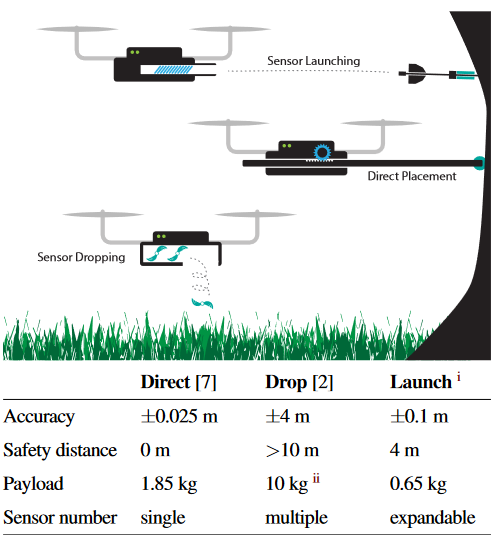
\includegraphics[width=0.48\textwidth]{Images/threeway.png}
    \caption{Different types of sensor placement from \cite{farinha2020unmanned}}
    \label{fig:threeway}
\end{figure}

The characteristics of each one of mentioned methods are shown in figure \ref{fig:threeway}.
We decided to go through with the Direct Placement strategy because despite its simplicity, it provides good accuracy and is able to place a large variety of payloads.\\

\subsection{Current State of the art for UAM}
There exists 2 main approaches for controls of unmanned aerial manipulators: The first one is the centralized approach where we consider the manipulator and the UAV as a whole; whereas in the decentralized approach, the manipulator controls and UAV control are independant problems.
In the case of the Sensor placement with a quadcopter, we use the centralized approach because the arm has no degree of freedom and the force exerted by the tip is coming from the thrust of the UAV.
The centralized approach is often built on top of a model-based full state control loop optimized with LQR (Linear–quadratic regulator) around some desired state. 
In \cite{ruggiero2018aerial}, the author present the current state of the research for UAMs.
An UAM can be divided into 4 elements: the UAV floating base (in our case, a quadcopter), the robotic arm, a sensor/gripper attached to the end of the arm (in our case, a sensor will be attached to the end of the arm), diverse sensors on UAV to handle perception (the depth camera).
While the state of the art approaches for UAV controllers are based on minimizing a state trajectory error, the planning strategy we will study next is based on velocity fields.
\subsection{Velocity field path-planning for single and multiple unmanned aerial vehicles}
In \cite{farinha2020unmanned}, the author presents a path-planning technique based on velocity fields generated from potentials solution of Laplace's equation.
Two different types of solution to potential $V$ for the Laplace 
\begin{align} % Use & sign to align, use \nonumber to write a line without number.
    \laplacian{V} &=0 \nonumber \\
    \frac{\partial^2 V}{\partial x^2}+\dpd[2]{V}{y} &=0 \label{eq:Laplace} % dpd = display mode partial derivative
\end{align}
equation are presented in this paper: Type 1 are irrotational solutions to generate sink and source fields and Type 2 solutions are used to build solenoidal fields.
\begin{align} % Use & sign to align, use \nonumber to write a line without number.
    {V}_{1} = {Q}_{1} \ln(({x}_{1}-\tilde{{x}_{1}})^2+({x}_{2}-\tilde{{x}_{2}})^2) \\ \label{eqn:potentiallogdistance}
    {V}_{2} = {Q}_{2} \arctan(\frac{({x}_{2}-\tilde{{x}_{2}})}{({x}_{1}-\tilde{{x}_{1}})})
\end{align}
where $({x}_{1},{x}_{2})$ is the position of the UAV, $(\tilde{{x}_{1}}, \tilde{{x}_{2}})$ is the position of the obstacle;
${V}_{1}$ and ${V}_{2}$ are respectively type 1 solution (source field) and type 2 solution (vortex field). \\
The author justifies the use of Laplace solution for building the velocity field for multiple reasons:
\begin{itemize}
    \item The use of Laplace solution for potential guarantees the uniqueness of the minimum in the field. 
    Specifically, the use of vortex function built from shaping function to circle around obstacle will
    ensure that only the goal point will be a minimum of the field and that the UAV will not get stuck at some local minimum. 
    As the author states, we can do an analogy to a famous strategy to find the exit of a maze: 
    by keeping a hand on a wall of the maze and walking while always touching the wall, we are ensured to find the end of the maze. 
    This is far from being an optimal solution, however, it can guarantee that the goal will be reached. 
    As a result, those solenoidal fields based on vortex function also provide active collision avoidance. 
    \item Scalar shaping functions are at the base of these methodology because by crafting them to match the shape of the obstacles, 
    we are able to generate corresponding vortex or repulsive functions for obstacles of any shape. 
    Since those functions are defined for each obstacle, it would be easy to reevaluate the field after addition or removal of an obstacle.
    \item Finally, irrotational solutions of the Laplace equation allow us to enforce an exclusion radius around obstacles (source field) and to direct the UAV in direction of the target point (sink field).
    The exclusion radius is encoded using the amplitude ${Q}_{1}$ of the irrotational field.
\end{itemize}

We can leverage these both types of potentials to derive a velocity field that will guide the UAV to the contact point without colliding with the surface.
For example, we could define the exclusion radius to be the distance between the centre of mass (CoM) of the quadcopter and its most distant part on the quadcopter. 

We will present the field we previously described with illustrations. 
\begin{figure}[h!]
    \centering
    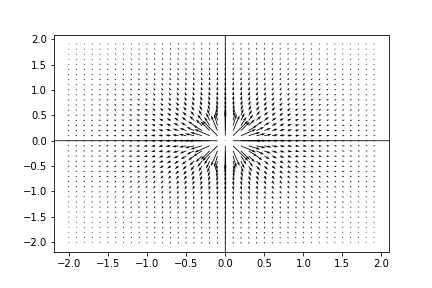
\includegraphics[width=0.48\textwidth]{Images/simplesource.png}
    \caption{Simple Type 1 irrotational source}
    \label{fig:simplesource}
\end{figure}
The field in figure \ref{fig:simplesource} was drawn by computing the gradient of $V_1$ with $(\tilde{{x}_{1}}, \tilde{{x}_{2}}) = (0,0)$.

\begin{figure}[h!]
    \centering
    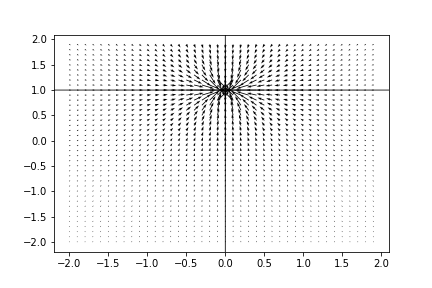
\includegraphics[width=0.48\textwidth]{Images/simplesink01.png}
    \caption{Simple Type 1 irrotational sink}
    \label{fig:simplesink}
\end{figure}
The field in figure \ref{fig:simplesink} is a sink field at $(0,1)$, it is similar to the source field in figure \ref{fig:simplesource} but with opposite sign.

\begin{figure}[h!]
    \centering
    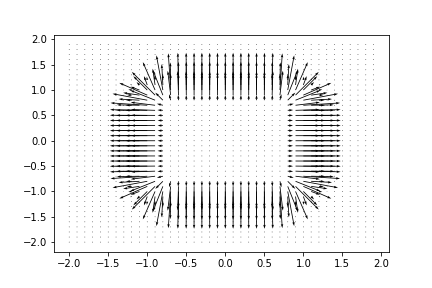
\includegraphics[width=0.48\textwidth]{Images/irrotafromshaping.png}
    \caption{irrotational field from shaping function}
    \label{fig:irrotafromshaping}
\end{figure}
The field in figure \ref{fig:irrotafromshaping} has been generated by computing the gradient of the shaping function of a superquadratic: 
\begin{align}
    H=(x_1-\tilde{{x}_{1}})^n+(x_2-\tilde{{x}_{2}})^n \\
    F=\frac{1}{1+(\frac{1}{L}H^{\frac{1}{n}})^m}
\end{align}
As stated in \cite{mcinnes2003velocity}, when $m\gg1$, the edge of the shaping function gets thinner. Higher values of $n$ result in more rectangular shapes whereas $n=2$ describes the shaping function of an infinite cylinder.

Both these fields are type 1 irrotational solutions of the Laplace equation.

By adding the irrotational sink from figure \ref{fig:simplesink} and the irrotational field from shaping function in figure \ref{fig:irrotafromshaping} we obtain a good representation in figure \ref{fig:irrotafromshapingwithsink} of what the velocity field will look like when close to the target point. 
\begin{figure}[h!]
    \centering
    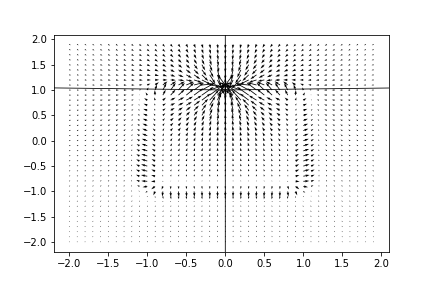
\includegraphics[width=0.48\textwidth]{Images/irrotashapingwithsink.png}
    \caption{irrotational field from shaping function with sink}
    \label{fig:irrotafromshapingwithsink}
\end{figure}

The shaping function is mainly used to generate a vortex field around an obstacle, as explained in the paper. It is given by: 
\begin{equation}
    v_2=-\frac{\partial{F}}{\partial{x_2}}e_1 + \frac{\partial{F}}{\partial{x_1}}e_2
\end{equation}
Here, $e_1$ and $e_2$ are an orthonormal basis. \\ 
We can see in figure \ref{fig:rotafromshaping} an example of vortex field around a super quadriatic.
\begin{figure}[h!]
    \centering
    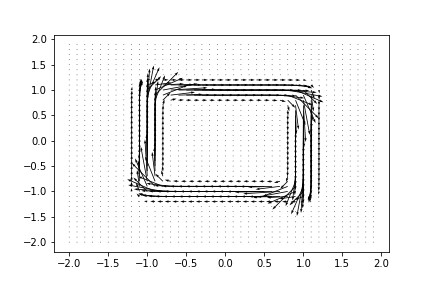
\includegraphics[width=0.48\textwidth]{Images/rotafromshaping.png}
    \caption{Solenoidal field from shaping function}
    \label{fig:rotafromshaping}
\end{figure}

\subsection{PID control \cite{johnson2005pid}}
In this subsection we will briefly describe what is a PID controller and how it is related to our task.
A PID (Proportional, Integral, Derivative) controller is a tool used to regulate the output $y(t)$ of a system to converge toward a setpoint value $SP(t)$ according to an error $e(t)=y(t)-SP(t)$, the time derivate of this error and the time integration of this error. 
It is defined by gain parameters $K_p$, $K_i$, $K_d$. 
\begin{figure}[h!]
    \centering
    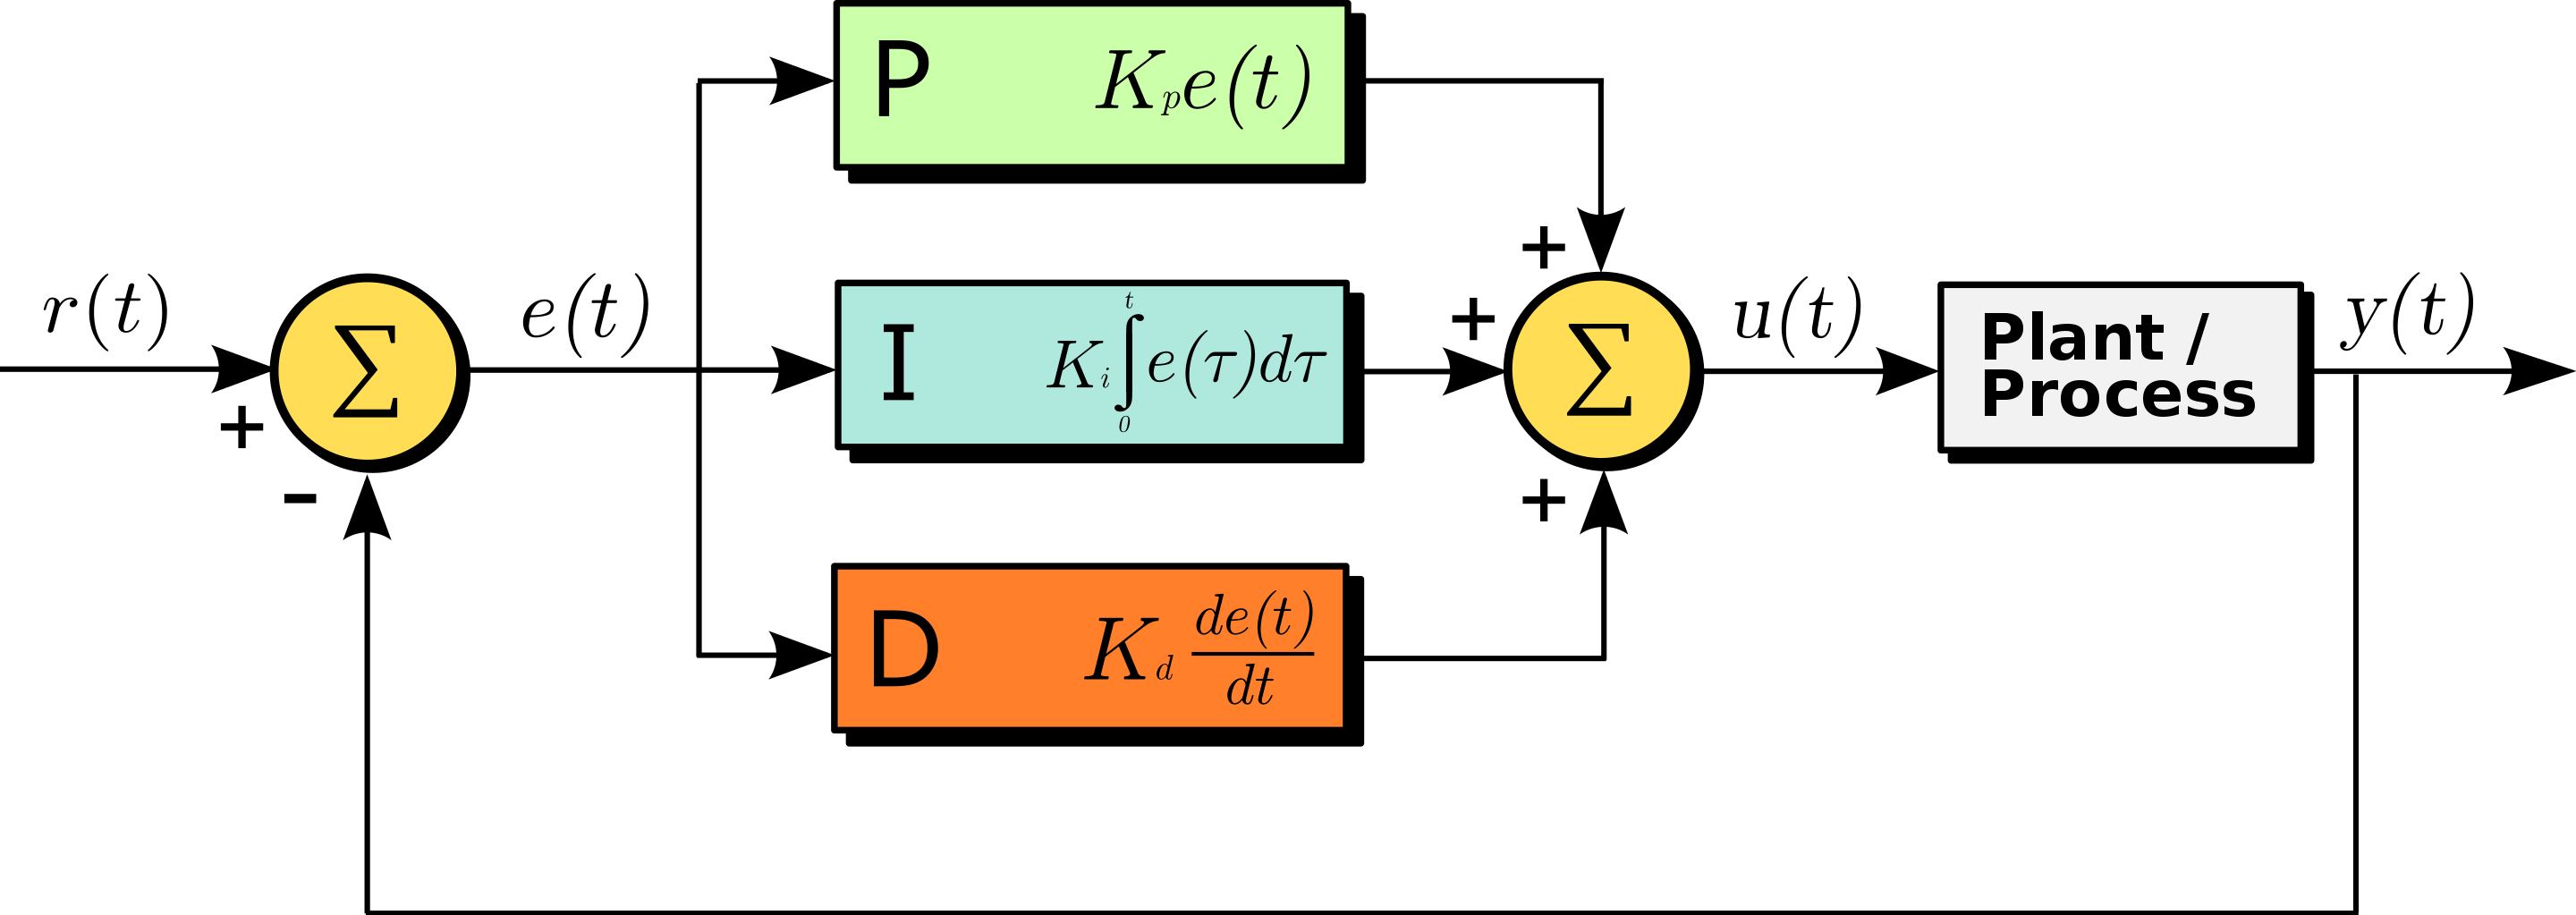
\includegraphics[width=0.48\textwidth]{Images/PID_en.svg.png}
    \caption{PID block diagram from Wikipedia}
    \label{fig:blockpid}
\end{figure}
The block diagram \ref{fig:blockpid} illustrate how this works. Let's assume a simple example where controller signals a new output every 1 second. 
Then we have : 
\begin{equation}
    u(t+1) = K_p e(t) + K_d \frac{de(t)}{dt} + K_i\int_0^te(t)dt
    \label{eqn:pid}
\end{equation}
The proportional gain is straightforward, we want to $y(t)$ to get closer to $SP(t)$.
However, in an inertial system, we might overshoot the setpoint when only using a proportional term. Therefore, to take into account how fast the error is decreasing (or increasing), we use a derivative term.
Finally, the integral term is to take into account historical value of the error and decrease the residual error.
The values of the gain parameters are application dependent.
In section 4, we will discuss using a PD controller (same as PID but without integral term) to control the attitude of the quadcopter in the Python implementation.
